\chapter{Padrões Criacionais}

\section{Factory Method}

O Factory Method define uma interface para criar 
objetos de forma que a responsabilidade de criação 
desses objetos seja da classe que irá implementá-la. 
Dessa forma, a interface não precisa saber qual 
classe deve ser instanciada, permitindo que versões 
diferentes ou implementações específicas de um mesmo 
tipo de objeto possam ser criadas.

Na figura \ref{fmethod_struct} é demonstrada 
a estrutura do padrão, onde a classe abstrata Creator 
define a operação abstrata que cria o objeto, 
o FactoryMethod. A classe ConcreteCreator 
implementa o FactoryMethod, criando um objeto 
do tipo ConcreteProduct, que é uma implementação 
específica de Product. Dessa forma, a classe 
abstrata Creator não precisa saber qual implementação 
de Product será criada.

\begin{figure}[htb]
	\caption{\label{fmethod_struct}Estrutura do Factory Method}
	\begin{center}
	    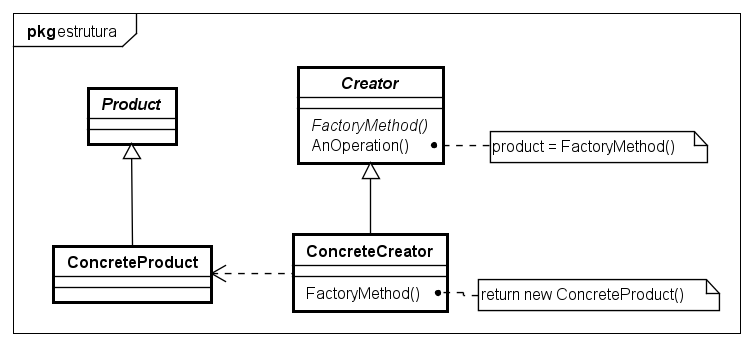
\includegraphics[scale=0.5]{5_padroes-contexto-funcional/5.1_criacionais/5.1.1_factory-method/factorymethod_struct.png}
	\end{center}
\end{figure}


\subsection*{Exemplo Orientado a Objetos}

Como exemplo é apresentado um \textit{framework} 
que cria e apresenta para o usuário múltiplos 
documentos. Para isso, a classe abstrata 
Application é definida com a operação abstrata 
CreateDocument e com uma lista de objetos 
que implementam a interface Document. A classe 
concreta MyDocument implementa Document e define 
um tipo de documento que pode ser utilizado pelo 
\textit{framework}, enquanto a classe concreta 
MyApplication herda de Application e implementa 
a operação CreateDocument para que ela crie 
um objeto do tipo MyDocument. O diagrama de classes 
para o exemplo pode ser visto na figura \ref{fmethod_example}, 
enquanto a implementação pode ser vista no 
código \ref{oofactory}.


\begin{figure}[htb]
	\caption{\label{fmethod_example}Exemplo de Factory Method}
	\begin{center}
	    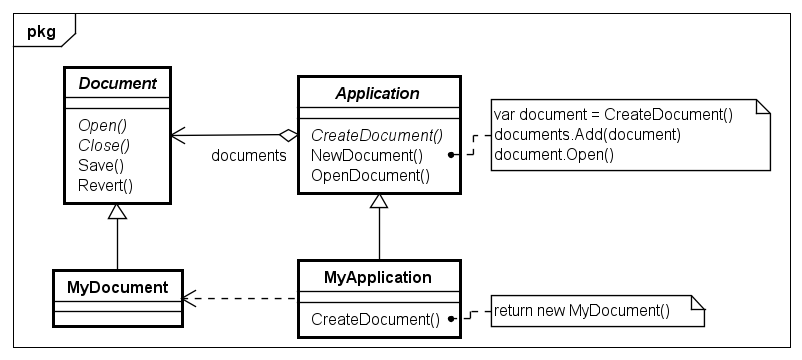
\includegraphics[scale=0.5]{5_padroes-contexto-funcional/5.1_criacionais/5.1.1_factory-method/factorymethod_exemplo.png}
	\end{center}
\end{figure}

\begin{lstlisting}[caption={Factory Method Orientado a Objetos},label=oofactory]
    
abstract class Document {
  def Open()
  def Close()
  def Save()
  def Revert()
}

abstract class Application {
  var documents : List[Document] = List()

  def CreateDocument() : Document

  def NewDocument() : Unit = {
    val doc = CreateDocument()
    this.documents = doc :: this.documents
    doc.Open()
  }

  def OpenDocument(): Unit = {
    println("Abre um documento")
  }
}

class MyApplication extends Application {
  def CreateDocument(): Document = new MyDocument()
}

class MyDocument extends Document {
  def Open(): Unit ={
    //...
  }

  def Close(): Unit ={
    //...
  }

  def Save(): Unit ={
    //...
  }

  def Revert(): Unit ={
    //...
  }
}

\end{lstlisting}

\subsection*{Contexto Funcional}



\begin{lstlisting}[caption={Factory Method Funcional},label=fpfactory]
    


\end{lstlisting}

